% defer/refcnt.tex
% mainfile: ../perfbook.tex
% SPDX-License-Identifier: CC-BY-SA-3.0

\section{Reference Counting}
\label{sec:defer:Reference Counting}
%
\epigraph{I am never letting you go!}{Unknown}

\begin{listing}
\input{CodeSamples/defer/route_refcnt@lookup.fcv}
\caption{Reference-Counted Pre-BSD Routing Table Lookup (BUGGY!!!)}
\label{lst:defer:Reference-Counted Pre-BSD Routing Table Lookup}
\end{listing}

\begin{listing}
\input{CodeSamples/defer/route_refcnt@add_del.fcv}
\caption{Reference-Counted Pre-BSD Routing Table Add\slash Delete (BUGGY!!!)}
\label{lst:defer:Reference-Counted Pre-BSD Routing Table Add/Delete}
\end{listing}

Reference counting tracks the number of references to a given object in
order to prevent that object from being prematurely freed.
As such, it has a long and honorable history of use dating back to
at least an early 1960s Weizenbaum
paper~\cite{Weizenbaum:1963:SLP:367593.367617}.
Weizenbaum discusses reference counting as if it was already well-known,
so it likely dates back to the 1950s or even to the 1940s.
And perhaps even further, given that people repairing large dangerous
machines have long used a mechanical reference-counting technique
implemented via padlocks.
Before entering the machine, each worker locks a padlock onto the
machine's on/off switch, thus preventing the machine from being powered
on while that worker is inside.
Reference counting is thus an excellent time-honored candidate for a
concurrent implementation of Pre-BSD routing.

To that end,
\cref{lst:defer:Reference-Counted Pre-BSD Routing Table Lookup}
shows data structures and the \co{route_lookup()} function and
\cref{lst:defer:Reference-Counted Pre-BSD Routing Table Add/Delete}
shows the \co{route_add()} and \co{route_del()} functions
(all at \path{route_refcnt.c}).
Since these algorithms are quite similar to the sequential algorithm
shown in
\cref{lst:defer:Sequential Pre-BSD Routing Table},
only the differences will be discussed.

\begin{fcvref}[ln:defer:route_refcnt:lookup:entry]
Starting with
\cref{lst:defer:Reference-Counted Pre-BSD Routing Table Lookup},
\clnref{refcnt} adds the actual reference counter,
\clnref{freed} adds a \co{->re_freed}
use-after-free check field,
\clnref{routelock} adds the \co{routelock} that will
be used to synchronize concurrent updates,
\end{fcvref}
\begin{fcvref}[ln:defer:route_refcnt:lookup:re_free]
and \clnrefrange{b}{e} add \co{re_free()}, which sets
\co{->re_freed}, enabling \co{route_lookup()} to check for
use-after-free bugs.
\end{fcvref}
\begin{fcvref}[ln:defer:route_refcnt:lookup:lookup]
In \co{route_lookup()} itself,
\clnrefrange{relprev:b}{relprev:e} release the reference
count of the prior element and free it if the count becomes zero,
and \clnrefrange{acq:b}{acq:e} acquire a reference on the new element,
with \clnref{check_uaf,abort} performing the use-after-free check.
\end{fcvref}

\QuickQuiz{
	Why bother with a use-after-free check?
}\QuickQuizAnswer{
	To greatly increase the probability of finding bugs.
	A small torture-test program
	(\path{routetorture.h}) that allocates and frees only
	one type of structure can tolerate a surprisingly
	large amount of use-after-free misbehavior.
	See \cref{fig:debugging:Number of Tests Required for 99 Percent Confidence Given Failure Rate}
	on \cpageref{fig:debugging:Number of Tests Required for 99 Percent Confidence Given Failure Rate}
	and the related discussion in
	\cref{sec:debugging:Hunting Heisenbugs}
	starting on
	\cpageref{sec:debugging:Hunting Heisenbugs}
	for more on the importance
	of increasing the probability of finding bugs.
}\QuickQuizEnd

\begin{fcvref}[ln:defer:route_refcnt:add_del]
In \cref{lst:defer:Reference-Counted Pre-BSD Routing Table Add/Delete},
\clnref{acq1,rel1,acq2,rel2,rel3} introduce locking to synchronize
concurrent updates.
\Clnref{init:freed} initializes the \co{->re_freed} use-after-free-check field,
and finally \clnrefrange{re_free:b}{re_free:e} invoke
\co{re_free()} if the new value of
the reference count is zero.
\end{fcvref}

\QuickQuiz{
	Why doesn't \co{route_del()} in
	\cref{lst:defer:Reference-Counted Pre-BSD Routing Table Add/Delete}
	use reference counts to
	protect the traversal to the element to be freed?
}\QuickQuizAnswer{
	Because the traversal is already protected by the lock, so
	no additional protection is required.
}\QuickQuizEnd

\begin{figure}
\centering
\resizebox{2.5in}{!}{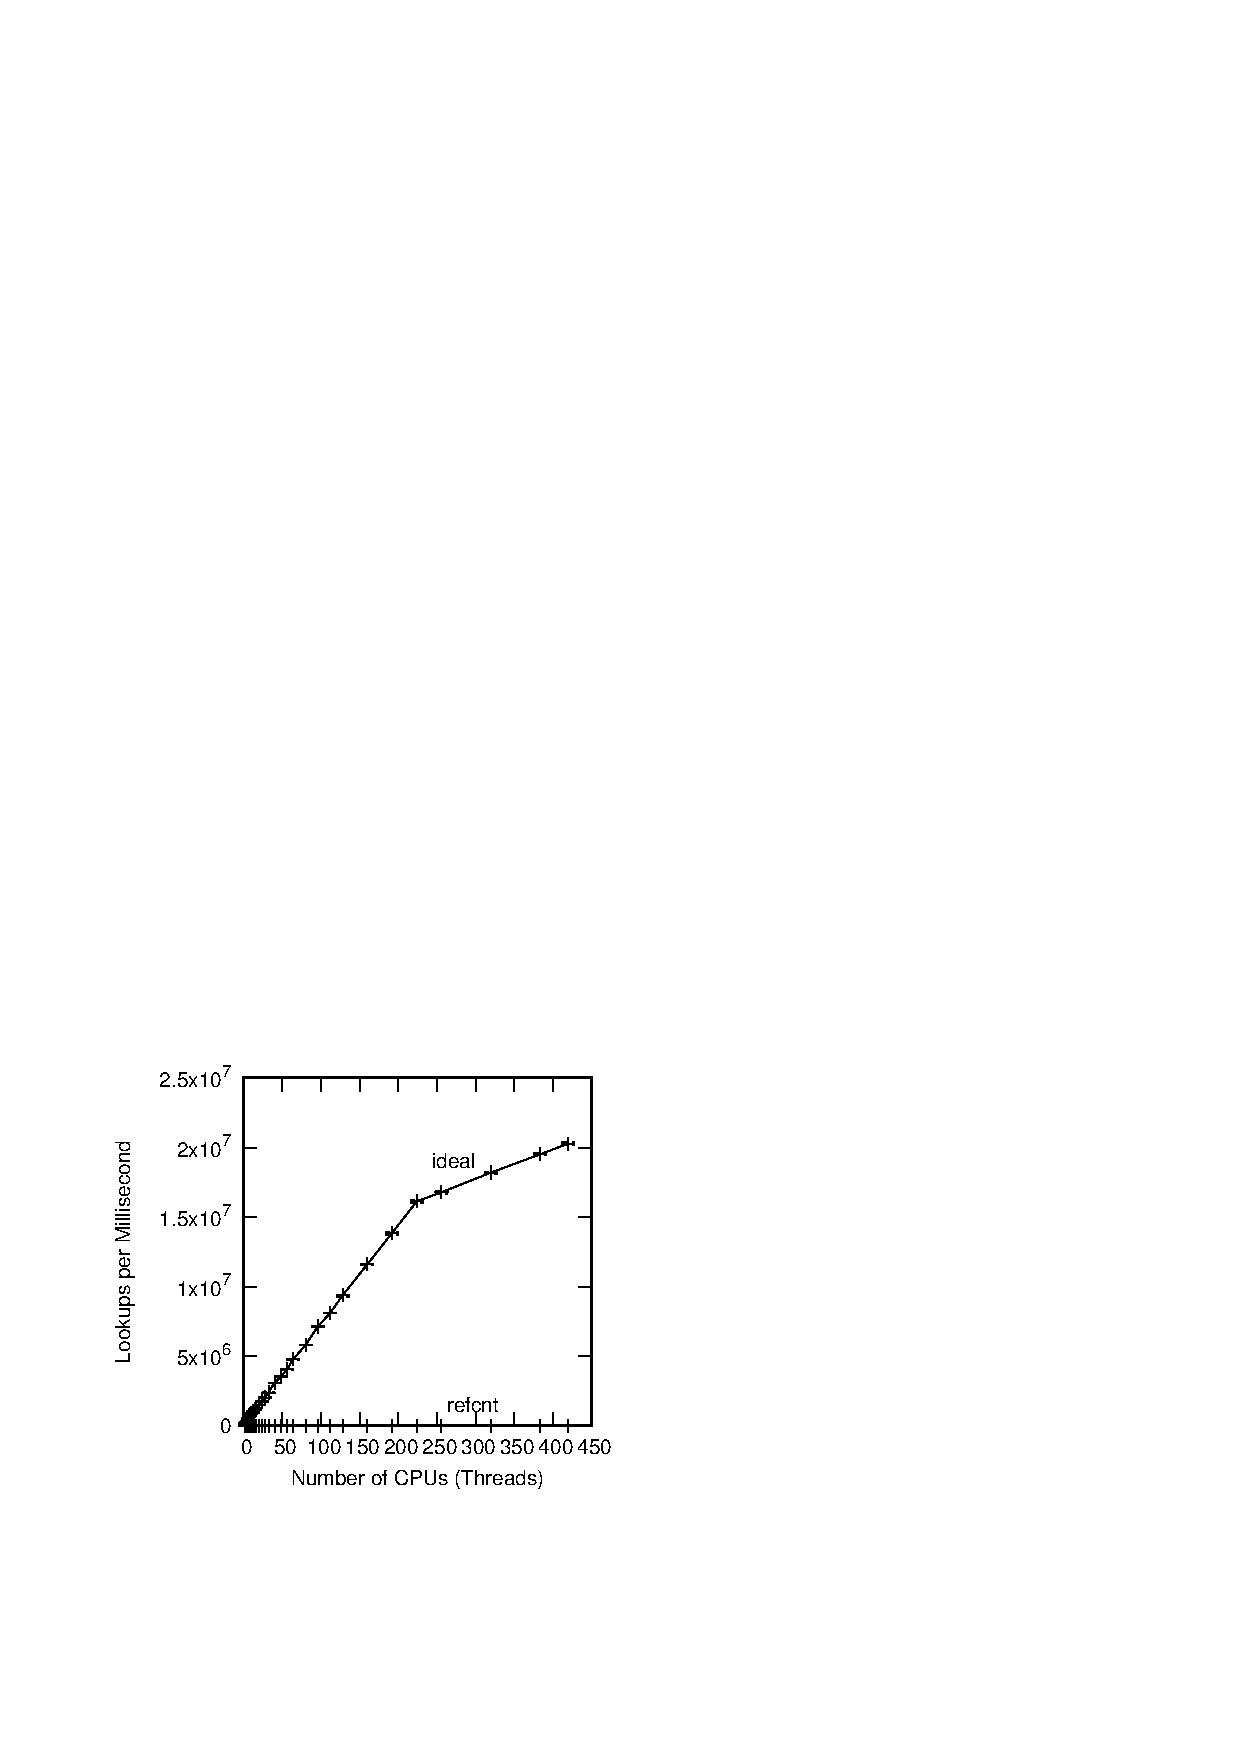
\includegraphics{CodeSamples/defer/perf-refcnt}}
\caption{Pre-BSD Routing Table Protected by Reference Counting}
\label{fig:defer:Pre-BSD Routing Table Protected by Reference Counting}
\end{figure}

\Cref{fig:defer:Pre-BSD Routing Table Protected by Reference Counting}
shows the performance and scalability of reference counting on a
read-only workload with a ten-element list running on an eight-socket
28-core-per-socket hyperthreaded 2.1\,GHz x86 system with a total of
448 hardware threads (\path{hps.2019.12.02a/lscpu.hps}).
The ``ideal'' trace was generated by running the sequential code shown in
\cref{lst:defer:Sequential Pre-BSD Routing Table},
which works only because this is a read-only workload.
The reference-counting performance is abysmal and its scalability even
more so, with the ``refcnt'' trace indistinguishable from the x-axis.
This should be no surprise in view of
\cref{chp:Hardware and its Habits}:
The reference-count acquisitions and releases have added frequent
shared-memory writes to an otherwise read-only workload, thus
incurring severe retribution from the laws of physics.
As well it should, given that all the wishful thinking in the world
is not going to increase the speed of light or decrease the size of
the atoms used in modern digital electronics.

\QuickQuizSeries{%
\QuickQuizB{
	Why the break in the ``ideal'' line  at 224 CPUs in
	\cref{fig:defer:Pre-BSD Routing Table Protected by Reference Counting}?
	Shouldn't it be a straight line?
}\QuickQuizAnswerB{
	The break is due to hyperthreading.
	On this particular system, the first hardware thread in each
	core within a socket have consecutive CPU numbers,
	followed by the first hardware threads in each core for the
	other sockets,
	and finally followed by the second hardware thread in each core
	on all the sockets.
	On this particular system, CPU numbers 0--27 are the first
	hardware threads in each of the 28 cores in the first socket,
	numbers 28--55 are the first hardware threads in each of the
	28 cores in the second socket, and so on, so that numbers 196--223
	are the first hardware threads in each of the 28 cores in
	the eighth socket.
	Then CPU numbers 224--251 are the second hardware threads in each 
	of the 28 cores of the first socket, numbers 252--279 are the
	second hardware threads in each of the 28 cores of the second
	socket, and so on until numbers 420--447 are the second hardware
	threads in each of the 28 cores of the eighth socket.

	Why does this matter?

	Because the two hardware threads of a given core share resources,
	and this workload seems to allow a single hardware thread to
	consume more than half of the relevant resources within its core.
	Therefore, adding the second hardware thread of that core adds
	less than one might hope.
	Other workloads might gain greater benefit from each core's
	second hardware thread, but much depends on the details of both
	the hardware and the workload.
}\QuickQuizEndB
%
\QuickQuizE{
	Shouldn't the refcnt trace in
	\cref{fig:defer:Pre-BSD Routing Table Protected by Reference Counting}
	be at least a little bit off of the x-axis???
}\QuickQuizAnswerE{
	Define ``a little bit.''

\begin{figure}
\centering
\resizebox{2.5in}{!}{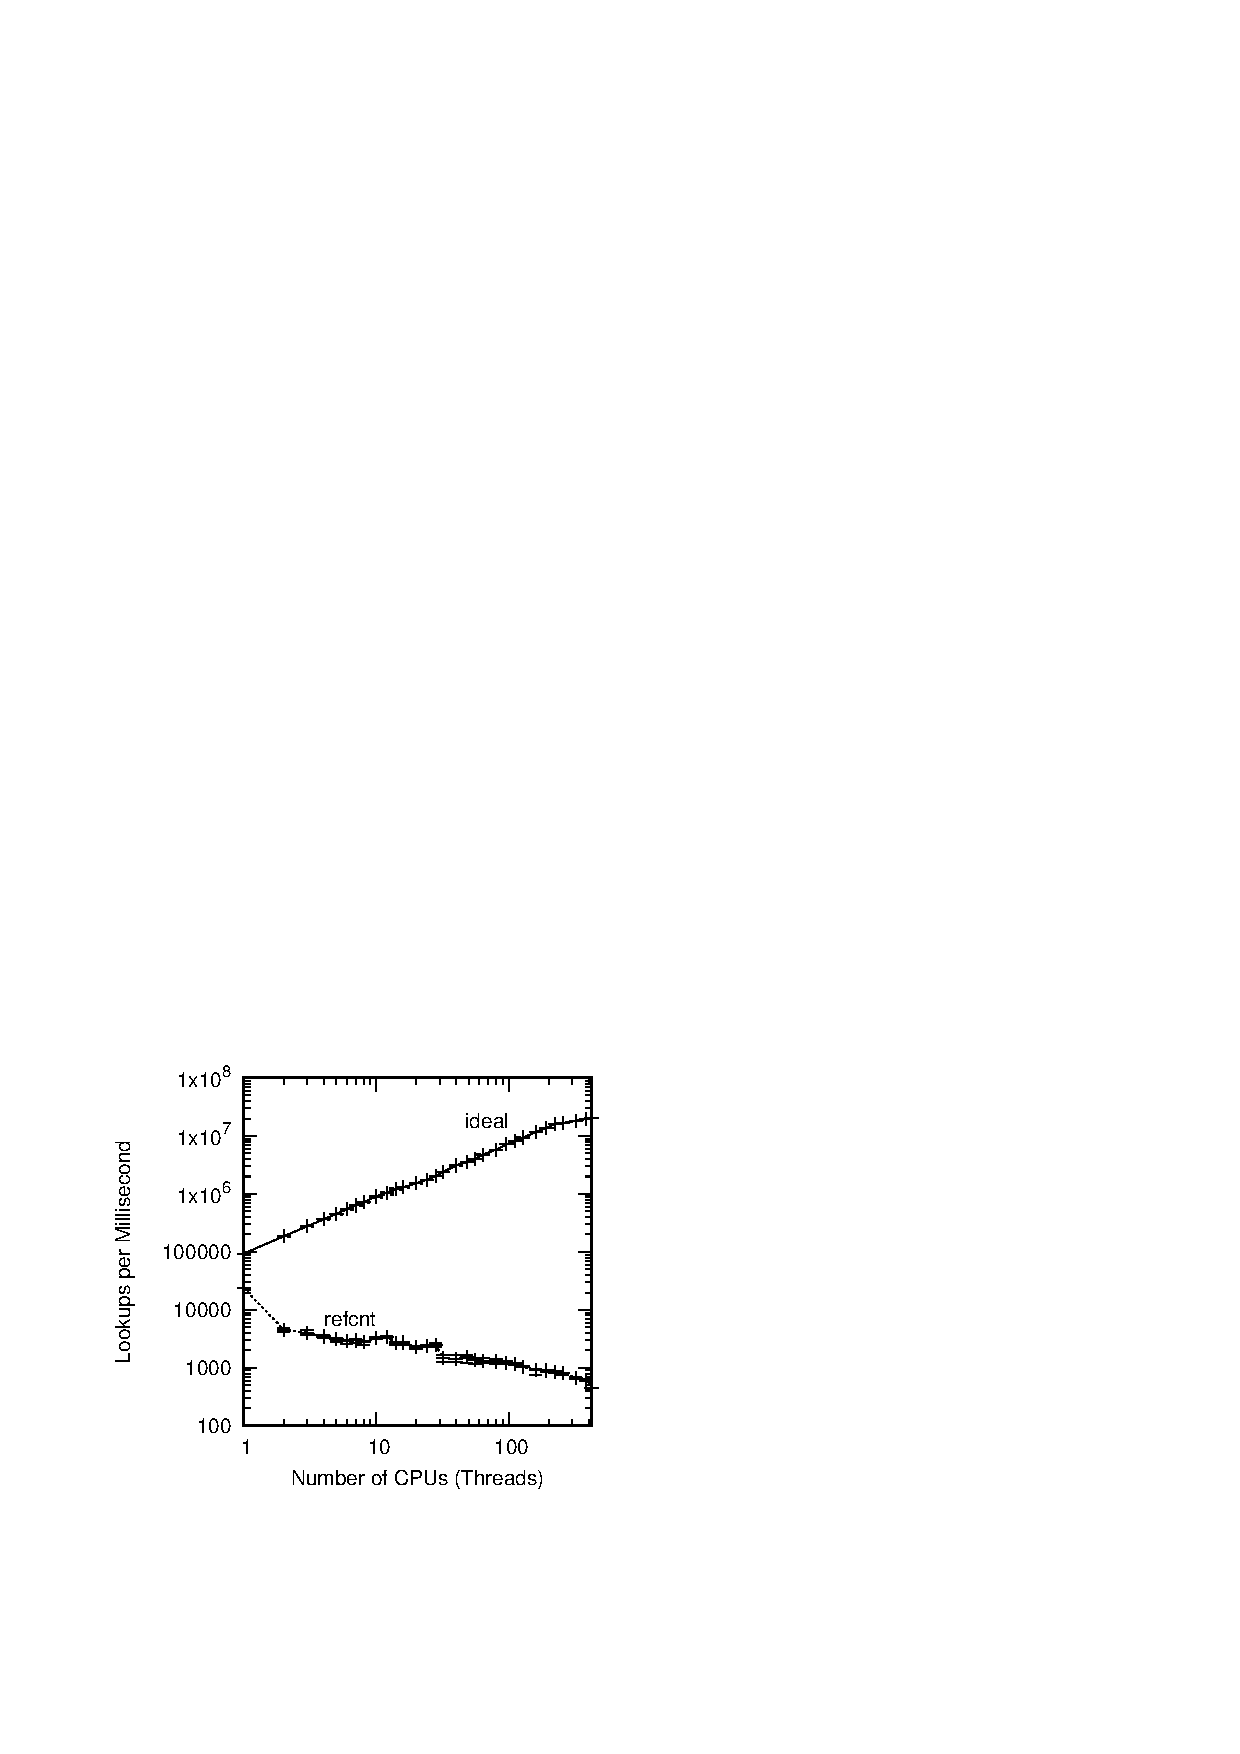
\includegraphics{CodeSamples/defer/perf-refcnt-logscale}}
\caption{Pre-BSD Routing Table Protected by Reference Counting, Log Scale}
\label{fig:defer:Pre-BSD Routing Table Protected by Reference Counting; Log Scale}
\end{figure}

	\Cref{fig:defer:Pre-BSD Routing Table Protected by Reference Counting; Log Scale}
	shows the same data, but on a log-log plot.
	As you can see, the refcnt line drops below 5,000 at two CPUs.
	This means that the refcnt performance at two CPUs is more than
	one thousand times smaller than the first y-axis tick of
	$5 \times 10^6$ in
	\cref{fig:defer:Pre-BSD Routing Table Protected by Reference Counting}.
	Therefore, the depiction of the performance of reference counting
	shown in
	\cref{fig:defer:Pre-BSD Routing Table Protected by Reference Counting}
	is all too accurate.
}\QuickQuizEndE
}

But it gets worse.

Running multiple updater threads repeatedly invoking
\co{route_add()} and \co{route_del()} will quickly encounter the
\co{abort()} statement on
\clnrefr{ln:defer:route_refcnt:lookup:lookup:abort} of
\cref{lst:defer:Reference-Counted Pre-BSD Routing Table Lookup},
which indicates a use-after-free bug.
This in turn means that the reference counts are not only profoundly
degrading scalability and performance, but also failing to provide
the needed protection.

One sequence of events leading to the use-after-free bug is as follows,
given the list shown in
\cref{fig:defer:Pre-BSD Packet Routing List}:

\begin{fcvref}[ln:defer:route_refcnt:lookup]
\begin{enumerate}
\item	Thread~A looks up address~42, reaching
	\clnref{lookup:check_NULL} of
	\co{route_lookup()} in
	\cref{lst:defer:Reference-Counted Pre-BSD Routing Table Lookup}.
	In other words, Thread~A has a pointer to the first element,
	but has not yet acquired a reference to it.
\item	Thread~B invokes \co{route_del()} in
	\cref{lst:defer:Reference-Counted Pre-BSD Routing Table Add/Delete}
	to delete the route entry for address~42.
	It completes successfully, and because this entry's \co{->re_refcnt}
	field was equal to the value one, it invokes
	\co{re_free()} to set the \co{->re_freed} field and to free the entry.
\item	Thread~A continues execution of \co{route_lookup()}.
	Its \co{rep} pointer is non-\co{NULL}, but
	\clnref{lookup:check_uaf} sees that
	its \co{->re_freed} field is non-zero,
	so \clnref{lookup:abort} invokes
	\co{abort()}.
\end{enumerate}
\end{fcvref}

The problem is that the reference count is located in the object
to be protected, but that means that there is no protection during
the instant in time when the reference count itself is being acquired!
This is the reference-counting counterpart of a locking issue noted
by Gamsa et al.~\cite{Gamsa99}.
One could imagine using a global lock or reference count to protect
the per-route-entry reference-count acquisition, but this would
result in severe contention issues.
Although algorithms exist that allow safe reference-count acquisition
in a concurrent environment~\cite{Valois95a}, they are not only extremely
complex and error-prone~\cite{MagedMichael95a}, but also provide
terrible performance and scalability~\cite{ThomasEHart2007a}.

In short, concurrency has most definitely reduced the usefulness
of reference counting!
Of course, as with other synchronization primitives, reference counts
also have well-known ease-of-use shortcomings.
These can result in memory leaks on the one hand or premature
freeing on the other.

\QuickQuiz{
	If concurrency has ``most definitely reduced the usefulness
	of reference counting'', why are there so many reference
	counters in the Linux kernel?
}\QuickQuizAnswer{
	That sentence did say ``reduced the usefulness'', not
	``eliminated the usefulness'', now didn't it?

	Please see
	\cref{sec:together:Refurbish Reference Counting},
	which discusses some of the techniques that the Linux kernel
	uses to take advantage of reference counting in a highly
	concurrent environment.
}\QuickQuizEnd

It is sometimes helpful to look at a problem in an entirely different
way in order to successfully solve it.
To this end, the next section describes what could be thought of as
an inside-out reference count that provides decent performance and
scalability.
